\documentclass[a4paper]{report}
% begin packages %
\usepackage[utf8]{inputenc}
\usepackage[usenames,dvipsnames]{xcolor} 	
\usepackage{listings}
\usepackage{amsmath}
\usepackage{amsfonts}
\usepackage[colorlinks=true, linkcolor=black, urlcolor=blue]{hyperref}
\usepackage{todonotes}
\usepackage{listings}
\usepackage{graphicx}
\usepackage[hypcap]{caption}
\usepackage{etoolbox}
\usepackage{xifthen}
%\usepackage{}
% end packages%

% setup style %
\setcounter{secnumdepth}{3}

\newcounter{testdescr}
\newcounter{testresult}
\DeclareCaptionFormat{Test}{Test \arabic{testdescr}: #3}
\DeclareCaptionFormat{Result}{Result \arabic{testresult}: #3}
%new commands

\newcommand{\HRule}{\rule{\linewidth}{0.5mm}}

\newcommand{\addassign}[2]{
	\mathrel{+}\;\!\!\mathrel{=}
}

\newcommand\numberthis{\addtocounter{equation}{1}\tag{\theequation}}

\newcommand{\testtable}[6][ ]{
	\begin{table}[!htbp]
		%\centering
		\stepcounter{testdescr}
		\begin{tabular}{| r p{9.5 cm} |}
			\hline
			\textbf{Test id:} & \textbf{\arabic{testdescr} - #2}\\
			\hline
			\emph{Measure:}		& #3\\
			\emph{Parameters:}	& #4\\
			\emph{Values:}		& #5\\
			\emph{Motivation:}		& #6\\
			\hline
		\end{tabular}
		\captionsetup{format=Test, aboveskip=5pt}
		\caption{#2}
		\label{test:\ifstrempty{#1}{\arabic{testdescr}}{#1}}
	\end{table}
}

\newcommand{\testresult}[3][]{
	\begin{figure}[!htbp]
		\centering
		\stepcounter{testresult}
		\makebox[\textwidth][c]{\includegraphics[width=1.2\textwidth]{figure/#2}}
		\caption{#3}
		\label{result:\ifstrempty{#1}{#2}{#1}}
	\end{figure}
}


%end new commands

\begin{document}
\lstset{
	language = c++,
	tabsize = 2,
	basicstyle = \footnotesize,
	backgroundcolor = \color{White},
	commentstyle = \color{OliveGreen},
	keywordstyle = \color{Blue},
	numberstyle = \color{Red},
	stringstyle = \color{BrickRed},
	frame=single,
	morekeywords = {
		cudaMemcpy,
		cudaMalloc,
		cufftResult,
		cufftPlanMany,
		cufftHandle,
		cufftType,
		cufftCreate,
		cufftExecC2C,
		cufftComplex,
		cudaEvent,
		cudaEvent\_t,
		cudaEventCreate,
		cudaEventRecord,
		cudaEventSynchronize,
		cudaEventElapsedTime,
		__global__,
		cudaMemcpyHostToDevice,
		cudaMemcpyDeviceToHost
	}
}


\pagenumbering{roman}
% % Front page
\begin{titlepage}
\begin{center}
\textsc{\LARGE TDT4501 - Computer Science, Specialization Project}\\[0.5 cm]

\textsc{\Large Fall 2014} \\[3cm]

\HRule \\[0.5cm]
\textsc{\huge \bfseries Particle-In-Cell Codes in CUDA}\\[0.5cm]
\HRule \\[1.5cm]

\large \emph{Author}: Olav Emil Eiksund\\[0.5cm]
\large \emph{Supervisor}: Anne Cathrine Elster

\vfill
{\large \today}
\end{center}
\end{titlepage}
% Abstract
\begin{abstract}
abstract content
\end{abstract}
%TOC and stuff
\tableofcontents
\listoffigures
%\listoftables
%
% Introduction
\chapter{Introduction}
\pagenumbering{arabic}

%%==%
This work has examined the application of GPU acceleration of \emph{Particle-In-Cell codes}, a particle simulation scheme.
Based on previous work using Pthreads, MPI and OpenMP, this work has used Nvidia's CUDA framework to parallelize the
simulation.

The particle-in-cell method consists of modeling charged particles in an electric field, with the solving of Poisson's
equation being an important step. With applications such as simulating the behavior of plasma or modeling particle
acceleration, there is an interest in performing these simulations with high accuracy, and with a good performance so as
to enable longer simulations etc.

Because of the limited resources available for this project, the scope has been more on issues encountered when developing
the simulator, rather than optimizing it for industrial or scientific use. Some questions serving as a goal for the project are:

\begin{enumerate}
	\renewcommand{\theenumi}{\alph{enumi}}
	\item Can Particle-In-Cell simulations be implemented in CUDA? Easily? \label{list:introduction-ease}
	\item Which issues are there when mapping the problem to CUDA? Which solutions or alternatives are available? \label{list:introduction-issues}
	\item Which parts of the simulation turn out to be critical paths? Can these parts of the code be improved further? \label{list:introduction-bottleneck}
\end{enumerate}

%==%
\section{Motivation}
\subsection{Why parallelize PIC codes?}
Particle-in-cell codes lends themselves reasonably well to parallelization, and the algorithm itself is quite simple,
with few steps. With few dependencies between elements, the sequential part of computation need not be to large, allowing
us to parallelize the algorithm without getting dominated by sequential code (see \ref{sec:background-speedup}).
\subsection{Why parallelize with GPGPU?}
GPGPU is a technology that makes use of a large number of slower cores to enable massive computational throughput, and
can be very cost effective compared to scaling with CPUs. Since many steps of the PIC algorithm consist of running the
same computation on all elements in a large two or three dimensional grid, GPGPU seems to be a great fit.

%==%
\section{Related Work}
A brief introduction to previous work that serves as a base for this project.

The overarching goal for the project has been to re-implement the algorithm from my advisor Anne Cathrine Elster's Ph.d.
Parallelization Issues and Particle-In-Cell Codes (Cornell, 1994) \cite{elster94} in CUDA. This work has therefore served
as an important theoretic background during development. Elster implemented a parallel PIC simulation with Pthreads
that was aimed at the distributed memory computer KSR1. Due to hardware limitations the implementation was in 2D.
The work explains the physics behind the simulation, and goes into some detail on how to optimize for performance on a
distributed shared memory machine. Elster also demonstrated how the simulation could reproduce physical phenomena such as
plasma wave oscillation when sufficient simulation parameters were chosen. While both SOR and FFT solvers \ref{sec:background-solvers}
are described and explained, the implementation made use of the FFT solver.

Jan C. Meyer \cite{meyer04} implemented PIC codes using MPI, as part of a project to compare cluster computer applicability to
supercomputer problems. The simulation is based on Elster's previous work, but uses the SOR solver instead, and rewrote
code from scratch due to problems in converting the existing work. Issues with the implementation are discussed, and it
is suggested that the implementation can be optimized quite a bit.

This was the initial goal of the masters project of Nils M. Larsgård \cite{larsgaard07}, but focus was switched to
optimizing Elster's original code. The main topic of the work is the performance of hybrid OpenMP/MPI code, and like
Meyer's code uses MPI for communication between nodes. While the FFTW library was used to improve the FFT solver
performance, OpenMP was used to accelerate the SOR solver within nodes.

%%==%
\section{Thesis Outline}
\paragraph{Introduction}
This section, an introduction to the work, and the motivation behind it.
\paragraph{Background}
Some background on the physics behind Particle-In-Cell codes, along with some insight into the two solvers used. In
addition of the recent history in parallel computing is given, with a special focus on GPGPU and CUDA.
\paragraph{Implementation}
Details about the implementation. Some known problems and issues are mentioned, as well as what can be done to improve
upon the current implementation.
\paragraph{Testing}
Various aspects of the implementation are benchmarked. Details about the testing methodology, and suggestions for further
tests to be done in the future.
\paragraph{Results}
Performance resuslts from benchmarks.
\paragraph{Discussion}
Interpretation of results and evaluation of the implementation. Existing flaws and potential for improvement is discussed.
\paragraph{Conclusion}
A summary of findings, and ideas for future work.
% Background
\chapter{Background}
This section will provide some details on the physics being modeled and the math behind the solvers used. In addition an
introduction to modern parallel programming and GPGPU will be given, with special focus on CUDA.

% ==Particle-In-Cell Codes== %
\section{Particle-In-Cell Codes}
Particle simulations attempt to model the behavior and interactions of particles and their forces, with applications in
for example fluid dynamics or studies of plasma, they tend to be very compute intensive. One type of simulations is
called Particle-in-cell codes.

Particle-in-cell simulations consist of finding the electrical charge distribution resulting from the particle charges,
solving the field to find the electrical potential, and move the particles based on the resulting electrical force and
their current velocity. The simulation is discrete in both time and space and sufficient resolution in either is
necessary to avoid aliasing, and properly model physical phenomena such as plasma wave oscillation.

% Subject of simulation %
\subsection{Subject of simulation}
The simulation models the behavior of charged particles in an electric field. In some PIC simulations a magnetic field
is present as well, but in this project the magnetic field is assumed to have no effect. Particles are modeled with
charge, mass, position and velocity.

% Equations %
\subsection{Discrete Model Equations}
The following equations form the basis of the simulation. The simulation procedure can be derived from these equations,
as seen below. For further detail on these equations see chapter 3 of \cite{elster94}. The only major difference is that
this explanation is given with three dimensional space.
\begin{equation} \label{eq:dm1} \nabla^2\Phi = -\frac{\rho}{\epsilon _0} \end{equation}
\begin{equation} \label{eq:dm2} \mathbf{E} = -\nabla\Phi \end{equation}
\begin{equation} \label{eq:dm3} \frac{dv}{dt} =\frac{q\mathbf{E}}{m} \end{equation}
\begin{equation} \label{eq:dm4} \frac{dx}{dt} = v \end{equation}

%%
\subsubsection{Poisson's equation}
Poisson's equation is a \emph{partial differential equation} (PDE) with uses in various disciplines, and specifically electrostatics.
The general form of the equation is $\Delta\phi = f$, which in euclidean space is equal to $\nabla^2\phi = f$. In 3D
Cartesian coordinates this becomes $\frac{\partial ^2\phi}{\partial ^2 x} + \frac{\partial^2\phi}{\partial ^2 y} + \frac{\partial ^2\phi}{\partial ^2 z}= f$.

The form found in equation \ref{eq:dm1} stems from Maxwell's equations, specifically Gauss's law for electricity. In
differential form written as
$$\nabla \cdot \mathbf{D} = \rho_f$$
the equation states that the divergence of the electric displacement field $\mathbf{D}$ is equal to the free charge
density $\rho_f$. With the assumption of no polarization or bound charges we have that
$$\mathbf{D} = \epsilon_0\mathbf{E}$$
Combining these leads us to
\begin{equation} \label{eq:poisson1} \nabla \cdot \mathbf{E} = \frac{\rho_f}{\epsilon_0} \end{equation}
We assume there is no changing magnetic field present, in which the Maxwell-Faraday Equation gives us
$$\nabla \times \mathbf{E} = -\frac{\partial\mathbf{B}}{\partial t}=0$$
and in turn equation \ref{eq:dm2}:
$$\mathbf{E}=-\nabla\Phi$$
Inserting this into equation \ref{eq:poisson1} we get:
$$\nabla \cdot \nabla \Phi = -\frac{\rho_f}{\epsilon_0}$$
or
$$ \nabla^2\Phi = -\frac{\rho_f}{\epsilon _0}$$
and in 3D form
$$\frac{\partial ^2\Phi}{\partial ^2 x} + \frac{\partial^2\Phi}{\partial ^2 y} + \frac{\partial ^2\Phi}{\partial ^2 z}= -\frac{\rho_f}{\epsilon _0}$$

By solving this equation using a 3D PDE solver we can find the electric potential $\Phi$ given the distribution of
electric charge $\rho_f$. This form of Poisson's equation is also known as Poisson's equation for electrostatics.

%%
\subsubsection{Electrical force from Potential}
Given the electric potential field $\Phi$ we want to determine the electrical force on a particle at position $p$. Using
equation \ref{eq:dm2} we can find the electric field $\mathbf{E}$
$$ \mathbf{E} = -\nabla\Phi $$
which is related to the electric force by
$$ \mathbf{F}_e = q\mathbf{E}$$

\paragraph{Discretized}
We can determine the field strength at each grid vertex using first order finite differences differences in each direction:
$$ \mathbf{E}_x(i, j, k) = -\frac{\Phi(i+1, j, k) - \Phi(i-1, j, k)}{h_x} = \frac{\Phi(i-1, j, k) - \Phi(i+1, j, k)}{h_x}$$
$$ \mathbf{E}_y(i, j, k) = \frac{\Phi(i, j-1, k) - \Phi(i, j+1, k)}{h_y} $$
$$ \mathbf{E}_z(i, j, k) = \frac{\Phi(i, j, k-1) - \Phi(i, j, k+1)}{h_z} $$
To find the electrical force on a particle we then need to interpolate the field strength at its position from its cell
vertices (see figure \ref{fig:trilinear}), and divide by the particle's charge.

%%
\subsubsection{Acceleration and velocity from Electrical force}
Given the force exerted on a particle we can use Newton's laws of motion to determine the effect on
it's velocity and position. We know that the particle's acceleration is
$$\mathbf{a} = \frac{\mathbf{F}}{m}$$
$$\mathbf{a} = \frac{d\mathbf{v}(t)}{dt}$$
$$\mathbf{v} = \frac{d\mathbf{x}(t)}{dt}$$

\paragraph{The leap frog method}
The particle's position and velocity is updated by integrating these equations, and in order to ensure a stable
simulation a leap frog integration method is used. By letting the position and velocity updates occur with half a
time-step's delay between, they "leap" over each other, resulting in a method more stable than the Euler method for
oscillations. The resulting discrete equations are:
$$v_{n+^{\!1}/_2} = v_{n-^{1\!}/_2} + \frac{\mathbf{F}(x, y, z)}{m}\cdot \Delta t$$
$$p_{n+1} = p_n + v_{n-^{1\!}/_2}\cdot \Delta t$$

\begin{figure}[!htbp]
	\centering
	\includegraphics[width=0.65\textwidth]{figure/leapfrog}
	\caption[Leap frog illustration]{An illustration showing how velocity and position are updated in a way causing them to "leap frog" over each
	other. Shown in transparent red are arrows illustrating $v_n$.}
	\label{fig:leapfrog}
\end{figure}

\subsubsection{Finding the charge distribution $\rho_f$}
In order to find the charge density on the grid we interpolate a particle's contribution to charge on it's neighboring
vertices, similarly to how the electrical field strength is interpolated. A particle's contribution to a vertex is
inversely proportional to their distance. The trilinear interpolation used is illustrated in figure \ref{fig:trilinear}

% Procedure %
\subsection{Procedure}
\begin{enumerate}
	\item Find charge density by accumulating particle charges on the grid.
	\item Solve for electrical potential using equation \ref{eq:dm1}.
	\item Derive electric field strength at all grid vertices from potential, using finite differences (\ref{eq:dm2}).
	\item Update particles:
	\begin{enumerate}
		\item Determine electrical field strength at particle position by trilinear interpolation of current cell vertex values.
		\item Using relation between acceleration, electrical force and electrical field strength, update particle velocity (\ref{eq:dm3}).
		\item Update particle position using updated velocity (\ref{eq:dm4}).
	\end{enumerate}
\end{enumerate}

% ==Solvers== %
\section{Solvers}\label{sec:background-solvers}
In order to handle different boundary conditions two different solvers have been implemented, one using the \emph{Fast Fourier
Transform}, the other based on \emph{Successive Over-Relaxation}. These are the same described by Elster in section 3.3 of \cite{elster94}.

% FFT %
\subsection{Fast Fourier Transform}
The fast Fourier transform is an efficient implementation of a discrete Fourier transform, which calculates a spectral
transform of a discrete signal. With extremely broad application, the FFT is known as one of the most important algorithms
in computer science today. A brief explanation of the FFT and it's background will be given.

\subsubsection*{Fourier Transform}
From a mathematical viewpoint the Fourier transform is an expression of a function of time as a function of frequency.
Related to the Fourier series, where a function can be approximated by a sum of sine and cosine terms, the Fourier
transform is similar to an infinite series, and the sum is replaced by an integral:
\begin{equation}
	\label{eq:ft}
	\hat{f}(\xi) = \int_{-\infty}^\infty f(x) e^{-2\pi i x \xi} dx
\end{equation}
Although equation \ref{eq:ft} shows a one dimensional transform this generalizes to any number of dimensions.

\subsubsection*{DFT}
A DFT shares most properties with the continuous Fourier transform, apart from being discrete in both input and output.
While the continuous transform ia a mathematical operation, the DFT has practical applications in ex. signal processing.
Compare equation \ref{eq:ft} for the Fourier transform with \ref{eq:dft} for the DFT:
\begin{equation}
	\label{eq:dft}
	X_k = \sum_{n=0}^{N-1} x_n \cdot e^{- 2\pi i k n / N}, k \in \mathbb{Z}
\end{equation}
$X$ is a length $N$ array of complex values, where each element $X_k$ represents one frequency bucket. A one dimensional DFT
 can be seen as finding the frequency distribution of the input signal, and as such each output element depends on the
 entire input array. The number of operations required for a full transformation is therefore $O(N^2)$.


\subsubsection*{Cooley-Tukey FFT algorithm}
The Cooley-Tukey FFT is of the most frequently used fast Fourier transforms. The FFT is an improvement over the DFT,
dividing a transform into a composite of smaller transforms recursively. The following example will divide by 2 (radix-2 FFT),
but any small prime can be used (mixed-radix FFT), letting the algorithm handle any length $n=2^a \cdot 3^b \cdot 5^c...$
The sum in equation \ref{eq:dft} is split into even and odd sums:
\begin{align*}
	X_k &= \sum_{n=0}^{N/2-1} x_{2n} \cdot e^{\frac{- 2\pi i k (2n)}{N}} + \sum_{n=0}^{N/2-1} x_{2n+1} \cdot e^{\frac{- 2\pi i k (2n+1)}{N}}\\
	X_k &= \sum_{n=0}^{N/2-1} x_{2n} \cdot e^{\frac{- 2\pi i k (2n)}{N}} + e^{\frac{- 2\pi i k}{N}} \cdot \sum_{n=0}^{N/2-1} x_{2n+1} \cdot e^{\frac{- 2\pi i k (2n)}{N}}\\
	X_k &= \sum_{n=0}^{N/2-1} x_{2n} \cdot e^{\frac{- 2\pi i k n}{N/2}} + e^{\frac{- 2\pi i k}{N}} \cdot \sum_{n=0}^{N/2-1} x_{2n+1} \cdot e^{\frac{- 2\pi i k n}{N/2}}
\end{align*}
	We can see that each sum corresponds to the transform of the odd and even parts of the input, with a common twiddle
	factor $e^{\frac{- 2\pi i k n}{N/2}}$. Since the input is assumed to be periodic either sum has the same value for $k=m$
	and $k=m+\frac{N}{2}$. Expressing the even sum as $C_k$ and the odd as $D_k$ we get:
\begin{align*}
	X_k &= C_k + e^{\frac{- 2\pi i k}{N}} \cdot D_k\\
	X_{k+\frac{N}{2}} &= C_{k+\frac{N}{2}} + e^{\frac{- 2\pi i}{N} (k+\frac{N}{2})} \cdot D_{k+\frac{N}{2}}\\
		&= C_k + e^{\frac{- 2\pi i}{N}k}\cdot e^{\frac{-2\pi i}{N}\cdot\frac{N}{2}} \cdot D_k\\
		&= C_k + e^{\frac{- 2\pi i}{N}k}\cdot e^{-\pi i} \cdot D_k\\
		&= C_k + e^{\frac{- 2\pi i}{N}k}\cdot (-1) \cdot D_k\\
		&= C_k - e^{\frac{- 2\pi i}{N}k}\cdot D_k
\end{align*}
 By reusing the values the number of computations is drastically reduced compared to the plain DFT.

\subsubsection*{Performance}
A main reason that the FFT has seen such widespread use is it's performance, sporting an $O\left(n\cdot log(n)\right)$
complexity, compared to the DFT at $O(n^2)$. As long as the dimensions of the input are multiples of small primes,
ideally a power of 2, the FFT is very efficient. For a number of reasons, ex. data alignment, this is often the case.

\subsubsection*{Properties/Issues}
An issue with the Fourier transform is aliasing, which may occur when there are signals in the input with frequencies
higher than the resolution of the transform. The result is that the transform interprets the samples from the signal at
a lower frequency. See figure \ref{fig:aliasing} for an illustration. The \emph{Nyquist theorem} states that to avoid
aliasing a sampling frequency at least twice the highest input frequency is needed. In cases where the highest input
frequency is unknown this can be hard to ensure, but aliasing will often be clearly visible in the output, for example as
procedural noise. Avoiding aliasing is one reason we want to maximize grid resolution in the implementation, since the
sampling frequency is the inverse of grid length in each direction, $f_x = n_x^{-1}$.
\begin{figure}[!htbp]
	\centering
	\includegraphics[width=\textwidth]{figure/aliasing}
	\caption[Aliasing]{An illustration of how a high frequency signal (green) can be misrepresented as a low frequency one (blue) due to insufficient sampling frequency.
	Samples shown as red circles.}
	\label{fig:aliasing}
\end{figure}

% SOR %
\subsection{SOR solver}
Successive over-relaxation is a scheme for iterative solvers, using a relaxation factor as a weight to ensure either
faster convergence. One assumes that the solution "lies further ahead", by weighting the value of neighboring
elements higher at the cost of an element's previous value.

\subsubsection*{System of linear equations}
A system of linear equations is the problem of finding $n$ unknowns $\mathbf{x}$, given $m$ linear equations on the form
$ a_{i1}x_1 + a_{i2}x_2 + a_{i3}x_3 + ... + a_{in}x_n = b_i $. In practice we are interested in solving systems where
$n \equiv m$ meaning there exists one unique solution. The simplest such system is $ax=b$, which is trivial in nature.
Practical applications can have systems with several thousand variables. Our problem can be represented as a two
dimensional system, with a relation between values in either direction.

\subsubsection*{The Jacobi method}
Among the most famous iterative linear solvers for systems of linear equations are the Jacobi and Gauss-Seidel methods.
Brief explanations of both follow. Assume a systen of linear equations:
\begin{align*}
	A \mathbf{x} &= \mathbf{b}\\
\intertext{A is split into a diagonal and remainder matrix.}
	A &= D+R\\
	A\mathbf{x} &= (D+R)\mathbf{x} = \mathbf{b}\\
	D\mathbf{x} &= \mathbf{b} - R\mathbf{x}\\
	\mathbf{x} &= D^{-1}(\mathbf{b} - R\mathbf{x})\\
\intertext{Iteration $n$ updates an element using the equation:}
	\mathbf{x}^{(n+1)} &= D^{-1}(\mathbf{b} - R\mathbf{x}^{(n)})\\
\end{align*}
Pseudocode using a 5 point stencil on a 2D matrix:
\begin{lstlisting}
while (err > threshold):
	for all i, j:
		updated[i, j] =
				(old[i-1, j] + old[i+1, j] + old[i, j-1] + old[i, j+1])/4
		
		err_ij = abs(updated[i,j] - old[i,j])
		if (err_ij > err):
			err = err_ij
\end{lstlisting}

\subsubsection*{Gauss-Seidel} 
Because a value depends on all neighboring old values, updates have to be written to a new matrix, resulting in a $2n$
storage requirement. The Gauss-Seidel method improves upon this by replacing reads to old values with updated ones, thus
allowing in-place updates. In addition this is shown to converge faster. Using the same matrix A,
\begin{align*}
	A &= L + D + U\\
\intertext{A is divided into lower triangle, diagonal, and upper triangle matrices.}
	A\mathbf{x} = (L + D + U)\mathbf{x} &= \mathbf{b}\\
	(L+D)\mathbf{x} &= \mathbf{b}-U\mathbf{x}\\
	\mathbf{x} &= (L+D)^{-1}(\mathbf{b}-U\mathbf{x})\\
\intertext{And as for Jacobi an element is updated as}
	\mathbf{x}^{(n+1)} &= (L+D)^{-1}(\mathbf{b}-U\mathbf{x}^{(n)})\\
\end{align*}
and pseudo-code for the same problem:
\begin{lstlisting}
while (err > threshold):
	for all i, j:
		updt[i, j] =
				(updt[i-1, j] + old[i+1, j] + updt[i, j-1] + old[i, j+1] )/4
		
		err_ij = abs(updated[i,j] - old[i,j])
		if (err_ij > err):
			err = err_ij
\end{lstlisting}

This way no subsequent calculations use $old[i, j]$ and updated $updt$ values can be written to the $old$ matrix. Gauss-Seidel
is therefore a more storage efficient method, important for large problems, and memory bound systems.

\subsubsection*{Over-relaxation}
A variant of Gauss-Seidel, successive over-relaxation has a minor modification which tends to result in faster convergence.
By using a weight $\omega$ (the \emph{relaxation factor}), the old value is used to either speed up convergence, or prevent divergence:
\begin{align*}
	A &= L + D + U\\
	(L + D + U)\mathbf{x} &= \mathbf{b}\\
	\omega(L + D + U)\mathbf{x} &= \omega\mathbf{b}\\
	\big[\omega L+ (\omega + 1 - 1)D\big]\mathbf{x} &= \omega\mathbf{b}-\omega U\mathbf{x}\\
	(\omega L + D)\mathbf{x} &= \omega\mathbf{b}-\big[\omega U + (\omega-1)D\big]\mathbf{x}\\
	\mathbf{x} &= (\omega L+D)^{-1}(\omega\mathbf{b}-\big[\omega U + (\omega-1)D\big]\mathbf{x})\\
	\mathbf{x}^{(n+1)} &= (\omega L+D)^{-1}(\omega\mathbf{b}-\big[\omega U + (\omega-1)D\big]\mathbf{x}^{(n)})\\
\end{align*}
\begin{lstlisting}
while (err > threshold):
	for all i, j:
		temp = (updt[i-1, j] + old[i+1, j] + updt[i, j-1] + old[i, j+1] )/4
		updt[i, j] = (omega-1) * old[i, j] + omega * temp
		
		err_ij = abs(updated[i,j] - old[i,j])
		if (err_ij > err):
			err = err_ij
\end{lstlisting}

The value of $\omega$ is used to control the influence the old value has on the new. $\omega = 1$ is the same as
Gauss-Seidel, $\omega = ^1\!/_2$ is to take the average of the old and updated values, while $\omega = 2$ would result in $ new = 2\cdot updated - old$.
For $\omega < 1$ change between iterations is diminished, and gives a lower chance of divergence. $\omega > 1$ places
more focus on neighboring values, and may speed up convergence. We want to speed up convergence, and good choice for
$\omega$ has been shown to lie around $1.78$. 

\subsubsection*{Parallelized - Red-Black coloring}
\label{sec:red-black}
A problem with the Gauss-Seidel method is the dependency between an update and those preceding it. Because $updated[i]$
depends on $updated[i-1]$, these cannot be calculated in parallel. The Jacobi method however has no dependencies to elements
from the same iteration, but cannot be done in-place. We can get the best of both worlds however, using a Red-Black
Jacobi method. By updating every other element in parallel, we avoid read-write conflicts, and no dependencies between
elements being updates, see figure \ref{fig:red-black}.

\begin{figure}[!htbp]
	\centering
	\includegraphics[width=0.6\textwidth]{figure/sor-red-black}
	\caption[Red-black ordering]{An example of 2D red-black coloring of a matrix. By first updating black, and then the red elements,
	calculations can be done in parallel, and in-place. As seen with the green stencil, the center element is only dependent on the its neighboring black elements, not on red ones.}
	\label{fig:red-black}
\end{figure}

% ==Parallel Computing== %
\section{Parallel Computing}
Parallel computing may refer to any form of processing in which multiple operations are performed concurrently. This can
range from vectorizing instructions to running ten thousands of threads on thousands of nodes on a supercomputer. A
short introduction to the history and motivation behind parallel computing will be given, as well as a measure of
performance for parallel computing.

\paragraph{Moore's law, limits of single core processing, and the rise of multi-core}
Well known to every computer scientist, Moore's law described the consistent increase in processing power since the
1970s. Performance increased along with transistor density, and was observed to double approximately every two years.
As long as performance could be increased by simply building a faster processor, interest in multi-core computing was
limited.
Three factors became readily visible during the early 2000s:
\begin{itemize}
	\item{The Memory Wall}
	Processor speeds increased faster than memory speeds, making it harder to hide memory latency. The result was that
	further increases in CPU clock speed would be lost waiting for memory.
	\item{The ILP Wall}
	While instruction level parallelism (ILP) had been used to hide the growing disparity between CPU and memory clock
	speed, it became harder to extract further instruction level parallelism from a single stream of instructions.
	\item{The Power Wall}
	$$U_{CPU voltage} = O(f_{CPU frequency})$$
	$$P_{CPU power consumption} = O(V^2_{CPU voltage})$$
	Because of these relationships, and the fact that CPU clock frequency has been doubling yearly, and number of
	transistors steadily increasing, CPUs were consuming a lot of power, and becoming very hot dissipating this energy.
	While the increase in voltage has been mitigated somewhat by the shrinking die size, the small transistors and low
	voltage causes issues like subthreshold leaking and electromigration to become more prominent. 
\end{itemize}
The result is that the cost of increasing performance while avoiding the power wall is too great, considering that
memory latency is the bottleneck.

Because of these issues the industry has shifted to multi-core computing as a way of further increasing performance. By
creating chips consisting of several smaller simpler processors rather than one large complex one, power consumption
and manufacturing costs is decreased, at the cost of being harder to program.

Another solution has been to offload work to hardware accelerators, such as graphics cards. This method, known as GPGPU
will be explained in more detail below.

\paragraph{Amdahl's law, Gustafson's law}\label{sec:background-speedup}
With the advent of parallel computing a new measure of performance is needed. while single core processing has a maximum
performance equal to $IPS = f_{clock} \cdot IPC$, the number of instructions per second is equal to the number of
instructions per clock cycle times the clock frequency. Assuming a fully parallelizable problem, the performance should
scale with the number of course, $IPS = n_{cores} \cdot f_{clock} \cdot IPC$. In reality however, not all parts of a
problem are easily parallelizable, often some setup or preprocessing has to be done sequentially. Because of this we
need a measure dependent upon the number of processors utilized, and the portion or the problem that is parallelizable.
In particular we want a measure of the speedup using $n$ processors instead of one, based on the formula:
$$S_n = \frac{T_1^{\,execution\,time}}{T_n^{\,execution\,time}}$$

\emph{Amdahl's law} gives an intuitive formula for the speedup of a program running on $n$ processors where $P_{sequential}$
is the sequential fraction of the execution time:
$$ T_n = T_1 \cdot (P_{sequential} + \frac{P_{parallel}}{n}) $$
$$ S_n = \frac{T_1}{T_n} = \frac{T_1}{T_1 \cdot (P_{sequential} + \frac{P_{parallel}}{n})} = \frac{1}{P_{sequential} + \frac{P_{parallel}}{n}}$$
This formula is useful in finding the potential speedup when parallelizing a sequential program, but as is evident, the
sequential part will quickly dominate the parallel part. By setting $n = \infty$ the formula becomes $S_\infty = \frac{1}{P_{sequential}}$,
and for a program with a 20\% sequential part the maximum speedup is 5. With $n=8$ this same problem would get a speedup
of $S_8 = \frac{1}{0.2 + \frac{0.8}{8}} = 1 / 0.3 = 3.33$, and with 16 cores the speedup would be $S_16 = 4$. Clearly
this does not scale well, and GPU computing with thousands of cores makes little sense.

The answer given in \emph{Gustafson's law} is that the approach to parallelizing the problem is wrong, and instead
defines the speedup as
$$ S_n = P_{sequential} + n \cdot P_{parallel}= n - P_{sequential} \cdot (n-1) $$
The elementary difference here is an assumption that the size of the parallel part of the computation scales linearly
with the number of processors. In other words, by increasing the problem size alojng with the number of processors, we
can keep improving the speedup without getting dominated by the serial part. One could also think of this as writing a
parallel program instead of converting a serial one, allowing the workload to be optimized for parallel computing. This
is also the clue GPGPU's potential.
% ...and anything else worth mentioning. %

% ==GPGPU== %
\section{GPGPU}
\emph{General-purpose computing on graphics processing units} (GPGPU) is a fairly recent trend in parallel computing,
where programs are accelerated by running heavy computation on a graphics processing unit. Characterized by a large
number of slower, cheaper cores, graphics cards today deliver massive parallelism to a standard desktop computer at low
cost.

% History %
\subsection{History}
Traditional graphics pipelines allowed only data to pass from the CPU to the GPU, where it would be processed in several
steps, rendered, and output to some display device. Around 2001 programmable shaders enabled researchers to experiment
with GPU computing, by defining data in terms of graphics primitives. In order to alleviate some of the trouble of
programming this way, GPU-specific languages and libraries were made, hiding the shader language from the programming.
One such language was Sh \cite{libsh}.

Coinciding with the industry's shift towards multicore/parallel programming, GPUs became increasingly powerful and easier
to develop for over the next few years. From 2006 GPUs shifted from graphics-specific pipelined devices towards generic
stream processing, with increasingly powerful parallelism as well as general programmability. Today GPUs are contending
with CPUs, offering a potentially much higher performance at the cost of some generality. For parallel applications, GPUs
offer a significantly cheaper option than the CPUs required to achieve the same performance, both in terms of value and
power budget. For this reason many current supercomputers are including GPUs to increase processing power per node,
with three among the top ten having Nvidia Tesla GPUs installed\cite{top500}. Of the 500
75 use accelerator technology, with 53 using GPUs.

Take for instance the Titan supercomputer by Cray at Oak Ridge National Laboratory, which took the lead on the TOP500 list in
November 2012, and uses Nvidia Tesla. Compared to their previous supercomputer Jaguar, performance increased from $2.3PF$
to $27PF$ while power increased from $7MW$ to $9MW$.\cite{nvidiasc14intro} This means more than a tenfold increase in performance at the cost
of only $1.3\times$ the power. Already ORN labs and Nvidia are cooperating to see similar scaling for their next
supercomputer Summit, aiming for a 2017 installation\cite{nvidiasc14intro}.

\subsection{Performance}
The \emph{Nvidia GeForce 8800 GTX} is a high end GPU from 2007 with a theoretical peak performance of 518.4 GFLOPS
\footnote{\url{http://www.techpowerup.com/gpudb/187/geforce-8800-gtx.html}} and a power consumption of $155W$.
A contemporary high end CPU, the \emph{Intel® Core™2 Extreme Processor QX9650} had a peak performance of $96GFLOPS$
\footnote{Assuming SSE: $4 cores \cdot 8 \frac{FLOPS}{cycle} \cdot 3.0GHz = 96GFLOPS$.} with a power consumption of
$130W$. See \url{http://ark.intel.com/products/33921/Intel-Core2-Extreme-Processor-QX9650-12M-Cache-3_00-GHz-1333-MHz-FSB}.

A high end consumer GPU in 2014, the \emph{GTX 980}, has a theoretical peak performance of $4612 GFLOPS$
\cite{maxwell},
drawing $165W$
\footnote{\url{http://www.geforce.com/hardware/desktop-gpus/geforce-gtx-980/specifications}}
and costs around 5000 NOK
\footnote{\url{https://www.komplett.no/search?q=GTX980}}.
In comparison Intel's current high end CPU, the \emph{Intel Core i7-5960X Extreme Edition}, has a theoretical peak performance of $768 GFLOPS$
\footnote{Assuming AVX and FMA: $8 cores \cdot 32 \frac{FLOPS}{cycle} \cdot 3.0GHz = 192GFLOPS$.\\See also
\url{http://www.pugetsystems.com/blog/2014/08/29/Linpack-performance-Haswell-E-Core-i7-5960X-and-5930K-594/} for a lower estimate.},
a power consumption of $140W$
\footnote{\url{http://ark.intel.com/products/82930/Intel-Core-i7-5960X-Processor-Extreme-Edition-20M-Cache-up-to-3_50-GHz}},
and a cost of ca 9500 NOK
\footnote{\url{https://www.komplett.no/intel-core-i7-5960x-extreme-edition/822376}}.

From these numbers it looks as if the GPU provides than five times the performance at half the cost, with only a
slightly higher power consumption. In reality the performance of either will be lower, and for double precision operations
the CPU performance will decrease a lot less than will the GPU's, but it is apparent that the GPU can provide relatively
cheap performance, and that the performance continues to improve. Note that the above are only estimates based on
specifications and not measured results, and that prices may vary between vendors and stores.

% ==CUDA== %
\section{CUDA}
The \emph{Compute Unified Device Architecture}, or CUDA for short, is a GPGPU computing platform. Developed by Nvidia
and introduced in 2006, CUDA is a relatively young technology, but has already seen employment in a number of applications
and research papers.

To develop for the CUDA platform one can use CUDA libraries, languages including the C/C++ and Fortan extensions and the
OpenCL framework, and compiler directives such as OpenACC/OpenMP \cite{nvidiaopenmp}.
In addition there exists third party wrappers for many other languages.

For this project the \emph{CUDA C/C++} is used, and will be reflected in the brief introduction below.
An introduction to what CUDA is by Nvidia can be found at \url{http://blogs.nvidia.com/blog/2012/09/10/what-is-cuda-2/}.
% Programming model %
\subsection{Programming CUDA}
The CUDA C/C++ has a few special features that sets it apart from standard C/C++. Most importantly, there is a
distinction between \emph{host} and \emph{device} code. Host code runs on the CPU and is responsible for calling device code. Device
code runs on the GPU, and can be recognized as functions with the \lstinline{__global__} qualifier. These functions are
known as kernels, and several instances are executed in parallel on the CUDA cores of the GPU.

Code is compiled using Nvidia's LLVM\footnote{See \url{http://llvm.org/}}-based compiler \emph{NVCC}. NVCC in turn uses
either the GNU compiler \emph{gcc} or the Microsoft Visual Studio compiler \emph{cl} to compile host code, while device
code is compiled to the \emph{ptx} assembler language \cite{nvcc}.
When the program is executed on a device the Nvidia graphics driver compiles the ptx code into a device specific binary \cite{nvptx}.

Below is an example of a CUDA kernel, and a call to this kernel:
\begin{lstlisting}
__global__ kernel(float a, float* x, float *y, float *out, int max)
{
	// Find the index of the current thread:
	int idx = blockIdx.x * blockDim.x + threadIdx.x;
	// Stay within bounds of the arrays:
	if(idx >= max)
		return;	
	// Perform computation:
	out[idx] = a * x[idx] + y[idx];
}

// Host code
int count = 20;
size_t size = count * sizeof(float)
float f = 0.25f;

float 
	*h_x, *h_y, *h_out;
	*d_x, *d_y, *d_out;
cudaMalloc(&d_x, size);
cudaMalloc(&d_y, size);
cudaMalloc(&d_out, size);

// Copy input arrays to device:
cudaMemcpy(d_x, h_x, size, cudaMemcpyHostToDevice)
cudaMemcpy(d_y, h_y, size, cudaMemcpyHostToDevice)

kernel<<<1, 32>>>(a, d_x, d_y, d_out, count);

// Copy result back to host:
cudaMemcpy(h_out, d_out, size, cudaMemcpyDeviceToHost)
\end{lstlisting}

This is a typical CUDA kernel call, although stripped of error checks and the like. We see that the host has to allocate
memory for device arrays, copy data to the device, launch the kernel and copy the result back.

In launching the kernel we see a deviation from standard C/C++ function calls, the \lstinline{<<<1, N>>>} part. These
are special parameters required by all kernels, specifying how the threads are structured, using the syntax\lstinline{<<<blocksInGrid, threadsInBlock>>>}.
Each of these accept a \lstinline{dim3} argument that specifies the length of blocks and grids in three dimensions.
Above only one value is given, specifying the x dimension while y and z default to 1.

In the kernel body we find a thread's rank within this structure though threadIdx and blockIdx, while gridDim and blockDim
correspond to the values given in \lstinline{<<<blocksInGrid, threadsInBlock>>>}. Threads are launched in \emph{warps},
groups of threads that execute concurrently on a core, and the number of threads we launch should always be a multiple
of the warp size, which is usually 32. Because of this some threads we launch may not have a designated element to work
on, and to avoid reading and writing out of bounds we check the thread index against the array size.

\begin{figure}[!htbp]
	\centering
	\includegraphics[width=0.65\textwidth]{figure/threads}
	\caption[Hierarchical structure of threads.]{The thread hierarchy in CUDA is illustrated above, with a grid containing several blocks, which themselves contain several threads.
	This configuration would be calles as \lstinline{<<<(3, 3, 1), (5, 5, 1)>>>}.}
	\label{fig:thread-hierarchy}
\end{figure}

% Memory %
\subsection{Memory}
GPU-accelerated programs tend to be very sensitive to memory accesses, and so it is very important to be conscious of
data locality when looking to optimize code. In CUDA there are three main levels of memory, global device memory, shared
block memory, and thread local memory. Using figure \ref{fig:thread-hierarchy} as an example, all threads (blue) have their
own local memory, registers, and all threads in a block (red) have access to a shared memory, while all blocks may access
global memory. The difference in memory latency between levels are in order of magnitude, so it is desirable to keep
data as close to the thread level as possible. Local and shared memory lifetime is restricted to a kernel launch, so to
keep results they have to be written to global memory.

In addition to these there is a constant memory which is read-only from device code, and texture memory which is
optimized for stencil access.

% cuFFT %
\subsection{cuFFT}
cuFFT is Nvidia's FFT framework for CUDA. It consists of the cuFFT and cuFFTW libraries, with the former designed with
GPUs in mind, and the latter serving as a porting tool for code using the well known FFTW library\footnote{\url{http://www.fftw.org/}}.
The cuFFT library is the one used in the implementation, and no further detail will be given on cuFFTW.

The library claims excellent performance for input sizes on the$n = 2^a \cdot 3^b \cdot 5^c \cdot 7^d$, and for prime
factors up to 127 it uses the efficient Cooley-Tukey algorithm. For other sizes it falls back on the less accurate Bluestein's
algorithm\cite[sec.~2.12]{cufft-doc} which handles large prime sizes better. Transforms of up to three dimensions are
supported, with a maximum of 512 million elements for single precision and 256 million elements in double precision
transforms, although limited by device memory and transform type (complex or real input etc.)\cite[sec.~1]{cufft-doc}.
% Implementation
\chapter{Implementation}
% ==Structure== %
Because the work this project is based on used double precision data types this is done here as well, to make sure
errors are not due to insufficient accuracy. A switch to single precision data types was left as a question to be
evaluated based on results from testing.

In contrast to the previous work however, this simulation is done in 3D, adding realism at the cost of accuracy. Adding
an additional dimension increases the number of cells by resolution in that dimension times the number of cells in the
plane. Because the memory usage and algorithm complexity increases, the resolution of each dimension will be limited.
A 3D grid of $256^3$ contains the same number of cells as a 2D grid at $4096^2$.

% % =Kernels= %
\section{Kernels}
A description of the kernels follow.

% % determineChargesFromPotential %
\subsection{determineChargesFromPotential}
The kernel determining the charge density of the mesh from particle charges. The contribution of a particle to each
vertex of its resident cell is found using trilinear interpolation, illustrated in fig. \ref{fig:trilinear}. The
distribution of a particle charge $\rho_p$ is as follows:
\begin{align*}
                \rho(i, j, k) \quad &+=\quad \frac{\rho_p }{ (h_x \cdot h_y \cdot h_z)} \cdot (h_x-a) \cdot (h_y-b) \cdot (h_z-c)\\
            \rho(i+1, j, k) \quad &+=\quad \frac {\rho_p }{ (h_x \cdot h_y \cdot h_z)} \cdot (h_x-a) \cdot b \cdot (h_z-c)         \\
            \rho(i, j+1, k) \quad &+=\quad \frac {\rho_p }{ (h_x \cdot h_y \cdot h_z)} \cdot a \cdot (h_y-b) \cdot (h_z-c)         \\
       \rho(i+1, j+1, k) \quad &+=\quad \frac{\rho_p }{ (h_x \cdot h_y \cdot h_z)} \cdot a \cdot b \cdot (h_z-c)                   \\
           \rho(i, j, k+1) \quad &+=\quad \frac{\rho_p }{ (h_x \cdot h_y \cdot h_z)} \cdot (h_x-a) \cdot (h_y-b) \cdot c         \\
      \rho(i+1, j, k+1) \quad &+= \quad \frac{\rho_p }{ (h_x \cdot h_y \cdot h_z)} \cdot (h_x-a) \cdot b \cdot c                   \\
      \rho(i, j+1, k+1) \quad &+= \quad \frac{\rho_p }{ (h_x \cdot h_y \cdot h_z)} \cdot a \cdot (h_y-b) \cdot c                   \\
 \rho(i+1, j+1, k+1) \quad &+= \quad \frac{\rho_p }{ (h_x \cdot h_y \cdot h_z)} \cdot a \cdot b \cdot c
\end{align*}
As can be seen, the contribution for a vertex is proportional to its distance to the particle compared to the other
vertices, the closest one receives the most charge and all contributions sums to $\rho_p$. Visualized in figure \ref{fig:trilinear},
dividing the cells along the interpolation lines, the contribution of a vertex is proportional to the volume of the
opposite sub-prism. We can see that the variable terms of the equations above give the volume, for instance
$\rho(i+1, j+1, k+1)$ has the term $a\cdot b\cdot c$ which is the volume of the prism in the opposite corner.

The kernel as is does not use shared memory to reduce memory latency, and it relies on slow atomic operations to avoid
write conflicts.

\begin{figure}
	\centering
	\includegraphics[width=0.8\textwidth]{figure/trilinear}
	\caption{Trilinear interpolation of particles with mesh vertices.}
	\label{fig:trilinear}
\end{figure}

% % electricFieldFromPotential %
\subsection{electricFieldFromPotential}
The electric field strength at a point is approximated as the difference in potential between it's neighbors, measured
separately in each dimension.
\begin{align*}
	E_x &= \Phi_{i+1} - \Phi_{i-1}\\
	E_y &= \Phi_{j+1} - \Phi_{j-1}\\
	E_z &= \Phi_{k+1} - \Phi_{k-1}
\end{align*}
The electric field is therefore stored as a vector at each point in the grid (array of structures).

\paragraph{electricFieldAtPoint} is a device helper function for doing trilinear interpolation of the electric field strength at some floating point
position. Similarly to the charge density calculations, field strength at a position is accumulated from cell vertices,
with contribution from each one proportional to the distance to it.

% % updateParticles %
\subsection{updateParticles}
\begin{lstlisting}
	ax = p.electricfield.x * cfg.charge_by_mass;
	prev = (1 - cfg.drag * cfg.ts);
	p.velocity.x = p.velocity.x * prev + ax * cfg.ts;
	p.position.x += p.velocity.x * cfg.ts;
\end{lstlisting}
The particle update kernel first finds the field electrical field strength at the particle's position using the helper
function electricFieldAtPoint, and then the acceleration using $a_p=\frac{F_e}{m_p} = \frac{E \cdot q_p}{m_p}$. Velocity and position
is updated through a leap frog method, where there is a $^{\Delta t}\!/_2$ delay between velocity and position updates.
$$ v^{n+ ^1\!/_2 } = v^{n+ ^1\!/_2 } + a^n \cdot \Delta t $$
$$ p^{n+1} = p^n + v^n \cdot \Delta t $$
The result is that a position update uses a velocity value that lies between the two points in time, an "average" value,
and similarly for velocity updates.


% =cuFFT= %
\section{cuFFT}
The FFT-based solver uses the cuFFT library, and this section will therefore focus on usage rather than implementation.

\subsection{FFT setup}
To run an FFT a plan has to be set up first, and stored using a cufftHandle. For single transforms with simple data
layouts the cufftPlan\#d() functions provide a simple interface for 1D, 2D and 3D transforms, while more complex setups
may need to use cufftPlanMany(). This function allows input and output  to be batched and strided data. All plans
specify the data types of the transform with options of \emph{real-to-complex}, \emph{complex-to-real}(implicitly an
inverse transform), or \emph{complex-to-complex}, and single or double precision. R stands for real, C for complex,
while D and Z are the same only for double precision.
\begin{lstlisting}
//cufftPlanMany signature
cufftResult cufftPlanMany(
	cufftHandle *plan,// Pointer to the plan
	int rank,					// dimensionality, (1, 2 or 3)
	int *n,						// n[i] = size of dimension i
	int *inembed,			// Size of dimensions in storage
	int istride,			// Distance between elements in inner dimension
	int idist,				// Distance between first elements in a batch
	int *onembed,			// Same as the above but for output
	int ostride,			// ...
	int odist,				// ...
	cufftType type,		// real or complex, single or double precision
	int batch					// multiple transforms with one call
);
\end{lstlisting}

\subsection{FFT call}
After the plan has been created, the transform can be executed using cufftExecX2X(). X2X may be either R2C, C2R, C2C,
D2Z, Z2D, Z2Z and must match the type parameter of the plan. In addition to the plan generated using cufftPlanXX(),
pointers to input and output data must ge supplied. For C2C and Z2Z an additional direction parameter must be set. R2C
is implicitly forward, Z2D is implicitly inverse and so on.
\begin{lstlisting}
//cufftExecC2C signature
cufftResult cufftExecC2C(
	cufftHandle plan,			// Plan generated as above
	cufftComplex *idata,	// Input data pointer
	cufftComplex *odata,	// output data pointer
	int direction					// Direction (forward/inverse)
);
\end{lstlisting}
\begin{lstlisting}
// Example cufft procedure
cufftHandle plan, iplan;
cufftCreate(&plan);
cufftCreate(&iplan);
cufftPlanMany(plan, ...); // Paln the transforms
cufftPlanMany(iplan, ...);
cufftExecR2C(plan, ...); // Forward transform
// ...
// Do something in spectral domain.
// ...
cufftExecC2R(iplan, ...); // Inverse transform
\end{lstlisting}

% solve %
\paragraph{solve}
After the data has been transformed using cufft, solving the for the field is done by multiplying each value by
$^1\!/_{k^2} $, and then scaling by $ ^1\!/_{\epsilon_0} $ to get $\Phi$.

$$ \frac{1}{{\epsilon_0 \cdot \left(
	\left(\frac{(2\pi \cdot \text{i} }{ L_x}\right)^2 + \left(\frac{2\pi \cdot \text{j} }{ L_y}\right)^2 + \left(\frac{2\pi \cdot \text{k} }{ L_z}\right)^2
\right)}} $$

 In addition, we need to normalize the transformation, scaling the elements by the size of the data set, which is
 $N_x \cdot N_y \cdot N_z$. The resulting computation is then to multiply the value at (i, j, k) by
 $$ \frac{1}{{4\pi^2 \cdot \epsilon_0 \cdot N_x \cdot N_y \cdot N_z \cdot \left(\, ^{\text{i}^2}\!/_{L_x^2} +\, ^{\text{j}^2}\!/_{L_y^2} +\, ^{\text{k}^2}\!/_{L_z^2}\right)}} $$
\begin{lstlisting}
scale_factor = 1/(eps_0 * 4*pi*pi * n.x * n.y * n.z);

double scale = scale_factor /
			(i*i/(l.x*l.x) + j*j/(l.y*l.y) + k*k/(l.z*l.z));

//Complex number:
row[i].x *= scale;
row[i].y *= scale;
\end{lstlisting}

% =SOR= %
\section{SOR}
From Gauss's law we have
\begin{align*}
	\nabla^2\Phi =& \frac{\partial^2\Phi}{\partial x^2} + \frac{\partial^2\Phi}{\partial y^2} + \frac{\partial^2\Phi}{\partial z^2} = - \frac{\rho_f}{\epsilon_0}\\
\intertext{This is approximated using second order finite differences.}
	\nabla^2\Phi \approx& \frac{ \Phi_{i-1} + \Phi_{i+1} + \Phi_{j-1} + \Phi_{j+1} + \Phi_{k-1} + \Phi_{k+1} - 6\Phi_{i, j, k}}{h_x \cdot h_y \cdot h_z} = -\frac{\rho_{i, j, k}}{\epsilon_0}\\
\intertext{We solve for $\Phi_{i, j, k}$}
	\Phi_{i, j, k} =& \frac{\rho_{i, j, k}\cdot\frac{h_x h_y h_z}{\epsilon_0} + \Phi_{i-1} + \Phi_{i+1} + \Phi_{j-1} + \Phi_{j+1} + \Phi_{k-1} + \Phi_{k+1}}{6}\\
\intertext{Over-relaxed updates use}
	\Phi_{i, j, k}^{(n+1)} =& (\omega-1)\Phi_{i, j, k}^{(n)} + \omega\cdot\frac{\Phi_{i-1}^{(n)} + \Phi_{i+1}^{(n)} + \Phi_{j-1}^{(n)} + \Phi_{j+1}^{(n)} + \Phi_{k-1}^{(n)} + \Phi_{k+1}^{(n)}}{6}\\
	\Phi_{i, j, k}^{(n+1)} =& \Phi_{i, j, k}^{(n)} + \numberthis \label{eqn:sor-update}\\
	&\; \omega \cdot \left( \frac{\Phi_{i-1}^{(n)} + \Phi_{i+1}^{(n)} + \Phi_{j-1^{(n)}} + \Phi_{j+1^{(n)}} + \Phi_{k-1}^{(n)} + \Phi_{k+1}^{(n)}}{6}-\Phi_{i, j,k}^{(n)} \right) 
\end{align*}
The SOR solver builds on the red-black Jacobi method described in \ref{sec:red-black}, using over relaxation to speed up
convergence. While previous work\cite[sec.~3.3.3]{elster94}\cite[sec.~2.7.2]{larsgaard07} used five-point stencils in a 2D solver, a seven-point
stencil is used to account for the z dimension, this being a 3D solver. For this solver boundary values are set equal to
the center value ($\Phi_{i, j, k}$).

As is, the kernel is run a fixed number of times, rather than checking the error. Every iteration the kernel is run
twice, once each for red and black colored tiles, allowing in-place updates in parallel.

% SOR kernel %
\paragraph{SOR kernels}
An initSOR kernel is run first, saturating the \emph{Phi} array with the appropriate values,
$$ \Phi_{i, j, k} = \frac{\rho_{i, j, k}\cdot h_x h_y h_z}{6 \cdot \epsilon_0} $$

When the SOR kernel itself is called, the \emph{k} index is calculated as follows, in order to implement red-black
coloring:
$$k = 2 \cdot Idx.z + (i + j + flag) \% 2 $$
where flag is 0 or 1 depending on whether red or black tiles are updated. The update itself uses equation \ref{eqn:sor-update}:

\begin{lstlisting}
	tmp = (left + right + down + up + front + back)/6;
	Phi[i][j][k] = center + cfg.omega * (tmp - center);
\end{lstlisting}


% =Setup= %
\section{Setup}\label{sec:implementation-setup}
The implementation currently uses parameters set in a getConfig() function, rather than with preprocessor macros. While
this prevents the compiler from optimizing certain calculations it allows parameters to be read in at runtime,
functionality that existed in Elster's original implementation, which this one it intended to be a CUDA version of.
Parameters that can be set and their default values for testing are shown in section \ref{sec:testing-parameters}.

All device memory allocations except that for the particle array use pitched pointers to ensure data alignment, helping
ensure coalesced memory accesses when possible. While the arrays probably could be reused to save space, such an
optimization is left for further improvements. For the current version the focus has been on ease of debugging and
understandability, for which separate arrays are a better fit.

Kernel grid and block settings (specified as \lstinline|kernel<<<grid, block>>>(...)|)
are chosen to achieve 256 threads per block, with a (256, 1, 1) configuration for particle-indexing kernels, and (16, 4, 4)
for field-indexing kernels. Since the particle array is one dimensional its setting is trivial, but the choice for the
three dimensional ones need some consideration. For the sake of coalesced memory access one would want threads to access
values that are sequential in the x-dimension, so it makes sense to have a wider x dimension. But if shared memory is
used to speed up computation and we want to do a border exchange, a square grid offers the fewest $^{neighbor}\!/_{element}$ ratio,
reducing the number of transfers relative to the number of in-block computations. In the implementation a value of 16 is
chosen to ensure 128-byte alignment ($16 \cdot sizeof(double) = 128$) while maximizing the block volume.

\section{Particle tracing}\label{sec:implementation-tracing}
Particle tracing is here implemented by copying the particle array from device to host every iteration. The host has a
$(N_{iterations}+1) \cdot N_{particles} \cdot sizeof(Particle)$ array, where each particle's data is stored for each
iteration. After the simulation loop has executed this array is used to output an xml file structured as follows:
\begin{lstlisting}[language=xml]
<root n_iterations="..." n_particles="..." particle_interval="...">
	<iteration time="...">
		<particle id="...">
			<position x="..." y="..." z="..."/>
			<velocity x="..." y="..." z="..."/>
			<electric x="..." y="..." z="..."/>
		<particle>
	</iteration>
</root>
\end{lstlisting}
This file is read by a python script using matplotlib to animate the movement of the particles. As of yet this script is
sensitive to the data volume, and works best with a reduced number of updates. Because of this, and in order to reduce
the performance hit associated with transferring the particle array every iteration, an interval between particle
transfers is used, $particle\_interval$. The exact interval used depends on the resolution needed to properly trace the
particles' movements, which is a function of the testing parameters and typical particle movement speed.

Another option to reduce memory transfer latency is to instead store the array on the device, and then transfer the
whole array after execution. For small values of $N_{particles}$, where the cost of initiating a transfer (API call etc.)
is significant compared to the actual data transfer, this would likely lead to some speedup since
$$T_{init} + T_{trans}(N_{trans} \cdot N_{particles}) <N_{trans} \cdot \left(T_{init} + T_{trans}(N_{particles})\right)$$.
For large values of $N_{particles}$ however this would be less pronounced, since $T_{init} << T_{trans}(N_{particles})$.
In addition, keeping a large array stored on the device consumes memory otherwise available to increase the problem size,
thus limiting the grid resolution $n_x, n_y, n_z$ and $N_{particles}$, based on the number of iterations. To get the
best of both worlds on could store a certain number of iterations' worth of data on the device, and then transfer them,
making room for further updates on the device. By selecting a transfer frequency so that 


% Testing
\chapter{Testing}

%==%
\section{Testing methodology, motivation and procedure}
In testing the implementation the goal is to see how performance is affected by various factors. This includes testing
for different problem configurations to see which parameters have the biggest impact, and testing runtime for the
different kernels to determine which ones among them are the most demanding.
The parameters that are tested for are \emph{number of iterations} $N_{iterations}$, \emph{grid resolution in all
dimensions}$n_x, n_y \text{and} n_z$, and \emph{number of particles} $N_{particles}$. For each of these different tests
are run in order to account for various effects\todo{elaborate?}. Several test also include variation in more than one
of these values so we can see combined effects.
\subsection{Procedure}
\label{sec:cuda-measure}
Kernel timing is done using the following procedure based on the example by Mark Harris from Nvidia on \href{http://devblogs.nvidia.com/parallelforall/how-implement-performance-metrics-cuda-cc/}{devblogs.nvidia.com/...}.
\begin{lstlisting}
	cudaEvent_t beginning, end;
	cudaEventCreate(&beginning);
	cudaEventCreate(&end);
	
	cudaMemcpy(...);
	
	cudaEventRecord(beginning);
	// Code that should be measured goes in here.
	kernel<<<...>>>(...);
	cudaEventRecord(end);
	
	cudaMemcpy(...);
	
	cudaEventSynchronize(end);
	float timing = 0.0f;
	cudaEventElapsedTime(&milliseconds, beginning, end);
\end{lstlisting}
The code above works in the following way: cudaEventRecord(beginning) records the time of the next event recorded, which
would be the kernel call. The next cudaEventRecord(end) records when the next cuda event occurs, which would be the
cudaMemcpy call. cudaEventSynchronize(end) blocks CPU execution until the event has been recorded, ensuring a correct
measurement. By placing the code to be measured between cudaEventRecord(beginning) and cudaEventRecord(end) we can find
$\Delta t = end - beginning$.

\todo[inline]{Describe how total execution time is measured.}

%%==%
\section{System configuration}
The test system configuration is given in the figures below. \todo{about additional test systems?}
\subsection{Hardware}
The relevant hardware of the test system is given in table \ref{tab:hardware}.
\begin{table}[h!]
\begin{sloppypar}
	\begin{tabular}{|| p{1cm} | p{5cm} | p{5cm} ||}
	\hline
		CPU:&		\href{http://ark.intel.com/products/65523}{Core i7-3770K,\newline Intel} &
			3.50GHz $\times$ 4(8) \\ \hline
		RAM:&	\href{http://www.corsair.com/en/vengeancer-16gb-dual-channel-ddr3-memory-kit-cmz16gx3m2a1600c9g}{Corsair Vengeance 16 GB}\cite{} &
			2 $\times$ 8192 MB DDR3 1600MHz, 667MHz max bandwidth\\ \hline
		MB:&		\href{http://www.asus.com/Motherboards/P8Z77V_PRO/}{P8Z77-V PRO,\newline ASUStek Computer Inc.} &
			-\\ \hline
		GPU:&		\href{http://www.gigabyte.com/products/product-page.aspx?pid=4319\#ov}{Nvidia GeForce 660ti, Gigabyte OC} &
			1344 Kepler CUDA Cores, 915Mhz, 2GB GDDR5\\ \hline
		PSU:&		\href{http://www.corsair.com/en/hx-series-hx650-power-supply-650-watt-80-plus-gold-certified-modular-psu}{650W, Corsair HX} &
			650W\\
	\hline
	\end{tabular}
\end{sloppypar}
\caption{Hardware used in testing.}
\label{tab:hardware}
\end{table}

\subsection{Software}
Relevant software is listed in table \ref{tab:software}, along with the version number.
\begin{table}[h!]
\begin{sloppypar}
	\begin{tabular}{|| p{3.5cm} | p{8cm} ||}
	\hline
		OS:& Windows 7 Professional, Service Pack 1\\
		C/C++ compiler:& MS C/C++ Optimizing Compiler v17.0.61030 x86\\
		CUDA Toolkit version:& 6.5\\
		CUDA compiler:& nvcc 6.5.13\\
		GeForce driver:& 344.75\\
	\hline
	\end{tabular}
\end{sloppypar}
\caption{Software used in testing.}
\label{tab:software}
\end{table}

%==%
\section{Test parameter values}
label{sec:test-parameters}
\subsection{Constants}
Most of the parameters remain more or less fixed across tests. This is mainly because while they affect the numerical
accuracy of the simulation, they do not affect runtime performance. The values selected for these parameters are mostly
the same as those used by Larsgaard \cite{larsgaard}.
\todo[inline]{Present parameters that remain constant across tests, along with reasoning behind the chosen value for each parameter.}

\begin{align*}
\intertext{\textbf{Physical constants}}
	\intertext{\textit{Value of $\pi$ used in calculations:}}
		\pi &= 3.14159265359,\\
	\intertext{\textit{Value of permittivity of free space (electric constant):}}
		\epsilon_0 &= 8.854187817 \cdot 10^{-12 } F/m,\\
	\intertext{\textit{Value of electron charge (unit charge?):}}
		e_{charge} &= -1.60217657 \cdot 10^{-19 } C,\\
	\intertext{\textit{Value of electron mass:}}
		e_{mass} &= 9.10938291 \cdot 10^{-31 } kg,\\
\intertext{\textbf{Simulation parameters}}
	\intertext{\textit{ Simulation grid size:}}
		L_x = L_y = L_z &= 0.2 m,\\
	\intertext{\textit{Time step between iterations:}}
		\Delta t &= 1 \cdot 10^{-6 } s,\\
	\intertext{\textit{Drasg term:}}
		d_{drag} &= 0,\\
\intertext{\textbf{SOR settings}}
	\intertext{\textit{SOR relaxation factor:}}
		\omega &= 1.78,\\
	\intertext{\textit{Error threshold for convergence (currently unused, fixed nr of iterations):}}
		Err_{threshold} &= 1 \cdot 10^{-9},\\
	\intertext{\textit{Number of SOR iterations run:}}
		N_{SOR\_iterations} &= 128,\\
\intertext{\textbf{Parameters that are set depending on the test are}}
	\intertext{\textit{Grid resolution (nr of points in each direction):}}
		n_x = n_y = n_z &= \text{default: } 64,\\
	\intertext{\textit{Simulation iterations run:}}
		N_{iterations} &= \text{default: } 2048,\\
	\intertext{\textit{Number of particles simulated:}}
		N_{particles} &= \text{default: } 256
\end{align*}

\subsection{Variables}
The testing parameters are $N_iterations$, $N_{particles}$ and $n_x,y,z$. The default value for these unless otherwise
is stated is $N_iterations = 2048$, $N_{particles} = 256$ and $n_x,y,z = 64$. these values are chosen because they are
small enough to run a large number of tests, while large enough to \todo{say more eloquently} represent a real scenario.
The default solver is chosen as the cuFFT based one.

\todo{Why are test values chosen the way they are?}

Certain simulation settings are derived from these terms, in particular the threadPerBlock and blockPerGrid settings for
each kernel. These depends on either the grid resolution or the particle count, as shown in section \ref{sec:setup}, and
while they are not testing parameters themselves, the fact that they change is one of the effects measured in the tests.

%==%
\section{Description of tests}
Descriptions of all tests done are given below. These include definitions of the value measured (performance etc.), the
parameters tested for (problem size etc.), the parameter values that will be tested, as wel as a brief description of
the motivation behind doing the specific test.
\subsection{Application runtime for different configurations}
Perhaps the most common measure of performance, the runtime of a program will be the focus of this test. Time will be
measured using CUDA events using the procedure given in section \ref{sec:cuda-measure} (see also
 \href{http://devblogs.nvidia.com/parallelforall/how-implement-performance-metrics-cuda-cc/}{devblogs.nvidia.com/...}).

\subsubsection{Number of iterations}
This test just shows the increase in runtime as a function of the number of iterations. Ideally this scales linearly
with $T(N_{iterations}) = N_{iterations}\cdot T(1)$, but in practice this may not be so, and this test could give a good
basis for interpreting the results for the tests below.

\testtable
	[iterations-total]
	{Iterations1}
	{ $T_{total}(N_{iterations}) -$ Total application runtime.}
	{$N_{iterations} -$ Number of iterations.}
	{$N_{iterations} = 2^k, k\in [0,15]$}
	{A simple measure of the application performance. Time spent doing setup and trace file writing will have less effect
	on the result as the number of iterations increase (see Gustafson's law, section \ref{sec:gustafson}).}

\testtable
	[iterations-simulation]
	{Iterations2}
	{$T_{simul}(N_{iterations}) -$ Simulation time, time spent in the simulation loop.}
	{$N_{iterations} -$ Number of iterations.}
	{$N_{iterations} = 2^k, k\in [0,15]$}
	{Only including the simulation loop should in theory result in runtime increasing linearly with number of iterations
	($T_{simul} \approx T_{iteration} \cdot N_{iterations}$), but factors such as memory usage might prove otherwise, and
	it could be interesting to see the result in any case.}

\subsubsection{Grid resolution}
The resolution of the simulation grid ais likely one of a few key factors in determining performance. While we would
usually set $n_x = n_y = n_z$ and the effect of these on simulation accuracy should be equal in theory, the way the
arrays are stored in memory is different. For instance any $n_x \in [1,16]$ would result in the same memory footprint
due to padding (here assuming elements 8 byte wide and a 128 byte alignment requirement).

\testtable
	[grid-isotropic]
	{Grid - Isotropic scaling of $n$}
	{$T(n_x = n_y = n_z) -$ Application runtime.}
	{$n_x, n_y, n_z -$ Resolution in each dimension.}
	{$n_x = n_y = n_z = 2^k, k\in [0,10]$}
	{Several of the kernels use one thread per grid element, and this metric is an important one. Two competing effects
	makes this an interesting one; a low resolution grid means less work to be done, potentially leaving multiprocessors on the
	card idle while reducing the number of memory accesses, but a high resolution one results in fewer particles per cell,
	thus potentially reducing write conflicts from particle-based kernels. See also test \ref{test:Particles2}}

\testtable
	[grid-one]
	{Grid - Scaling of $n$ along one dimension.}
	{$T(n_x = n_y, n_z) -$ Application runtime.}
	{$n_z -$ Resolution in z dimension.}
	{$n_x = n_y \in (4, 16, 64, 256, 1024)$\newline
	 $n_z = 2^m, m\in [0,11]$}
	{Here we test the effects on performance of scaling $n$ along a single dimension, for different configurations of the
	other two dimensions. \\todo\{purpose\}}
	\todo{Should maybe test $n_x$ instead since $n_x$ < 512 wastes memory.}

\testtable
	[grid-odd]
	{Grid - Odd valued $n$}
	{$T(n_x = n_y = n_z) -$ Application runtime.}
	{$n_x, n_y, n_z -$ Resolution in each dimension.}
	{$n_x=n_y=n_z \in (5, 11, 23, 47, 97, 205, 429, 901)$
	  $n_x=n_y=n_z \in (6, 12, 26, 50, 102, 210, 436, 908)$}
	{By testing for some arbitrarily chosen odd numbers ($n\approx 2.1^k$), as well as some non-power of two even number on
	a similar scale as test \ref{test:grid-isotropic}, we should be able to compare the performance. The data gathered in this test
	should help generalize the other results, where power of two sizes are used.}

\subsubsection{Particle count}
First a measure of the impact the number of particles has on execution time, and then we see how different particle
counts perform for different grid resolutions.
\testtable
	[particle-standard]
	{Particles1}
	{$T(N_{particles}) -$ Application runtime.}
	{$N_{particles} -$ Number of particles.}
	{$N_{particles} = 2^k, k\in [2, 12]$}
	{The number of particles affect device saturation; few particles mean less work to be done, fewer competing reads/writes,
	  while a higher number of particles mean a larger number of multiprocessors will be kept busy.}

\testtable
	[particle-by-resolution]
	{Particles2}
	{$T(N_{particles}, n) -$ Application runtime.}
	{$N_{particles} -$ Number of particles.\newline
	  $n_x = n_y = n_z -$ Resolution in each dimension.}
	{$N_{particles} = 2^k, k\in [2, 12]$\newline
	  $n_x = n_y = n_z \in (16, 64, 256, 1024)$}
	{It can be interesting to see how particle number and grid resolution together affect performance, such as which
	  parameter affects performance the most. Given that the complexity of several operations is $O(n_x\cdot n_y \cdot n_z \cdot N_{particles})$
	  makes it interesting to see how performance scales when both are increased.}

\subsection{Comparison}
Solver performance.\todo{write}
\testtable
	[solver]
	{Solver}
	{$T_{solver}(Solver, n) -$ Solver execution time}
	{The type of solver used.\newline
	  $n -$ Grid resolution.}
	{Solver $-$ cuFFT-based solver, SOR-solver.\newline
	  $n \in(16, 64, 256, 1024)$}
	{By testing both solvers for various problem sizes we can get a measure of how well they scale, as well as which of them
	  offers better performance.}
	  
\subsection{Kernel runtimes}
This test involves measuring runtime for each kernel as functions of resolution and particle count.\todo{how/why?}
\testtable
	[kernel]
	{Kernel}
	{$T_{kernel}(n, N_{particles}) -$ Kernel execution time.}
	{$n_x, n_y, n_z -$ Grid resolution.\newline
	  $N_{particles} -$ Number of particles.}
	{$n\in(16, 64, 256, 1024)$\newline
	  $N_{particles} \in (16, 64, 256, 1024)$}
	{Examining the performance for the different kernels for various configurations of particles and resolution, we may be
	able to identify potential bottlenecks. These results may assist in explaining global results above.}

%==%
\section{Suggestions for further testing}
\subsection{Solver}
It would be useful to measure which of the two solvers offer better accuracy per performance. A test here could be to
set the number of SOR iterations so both solver use the same amount of time and then compare the numerical accuracy of
the results, but to do this we need to be able to tell which solver gives the best result, knowledge I do not have at
the present.\todo{OBS! FFT give exact answer, The question is, can the SOR solver give a "good enough" answer with less work? This test is still useful in this regard.}

Assuming that the FFT as an exact solver gives the correct answer, we could run both and then find a measure of the
error by taking the average of the difference between the result for each element. By plotting this measure against grid
resolution and SOR iterations we could study how these increase the accuracy of the SOR. Combining this with a plot of
performance as a function of SOR iterations and grid resolution, we could see accuracy gain compared to performance loss,
an interesting metric.

\subsection{Single precision data type}
If the implementation is extended to include an option of using single precision data, it would be useful to test the
speedup this would gain us, as well as the inevitable loss of accuracy. The results of these tests could then help
give an idea of the tradeoff involved in choosing one or the other.

For the single precision implementation we would also want to run most of the tests described above. At least for the
GeForce series of GPUs, throughput for single precision operations is significantly higher than for double precision
operations, more so than the reduction in bandwidth congestion. For this reason memory latency could become even more of
a factor, potentially reducing actual speedup.
\todo[inline]{Refer to the above in discussion, and refer to background material in the above.}

\subsection{System}Other tests that could be of interest are comparisons between running the same configuration on different systems. In
particular this goes for the GPU involved. The Tesla series of GPUs have significantly better double precision capabilities
compared to the GeForce series, relative to their single precision performance. A configuration that would fit on both
systems should perform better on the Tesla because of the number of available double precision floating point units,
even taking into account core, memory and bus clock speeds.
%==%

% Results
\chapter{Results}
This section will present some results from testing, in the form of 2D and 3D plots as appropriate, along with a brief
interpretation of the data.

All results are timed as described in section \ref{sec:testing-methodology}. Python with numpy and matplotlib is used to
present the data in the diagrams below. Runtime is measured in milliseconds, and unless otherwise specified is the time
taken for one iterations of the simulation, or one run through the tested code.

\section{Number of iterations}
\testresult{iterations2}{Simulation loop runtime as a function of $N_{iterations}$.}

As be expected the simulation runtime scaled linearly with the number of iterations, as can be seen on figure \ref{result:iterations2}.
Runtime was approximately $1.35\frac{\mathit{milliseconds}}{\mathit{iteration}}$.

\section{Grid resolution}
\testresult{grid1}{Simulation iteration runtime as a function of grid resolution. Isotropic.}
\testresult{grid2}{Runtime as a function of grid resolution, with scaling along z axis.}
\testresult{grid3b}{Runtime as a function of grid resolution, isotropic, odd valued size.}
\testresult{grid3a}{Runtime as a function of grid resolution, isotropic, even valued size.}
	
The isotropic scaling of grid resolution is shown in figure \ref{result:grid1}. We see result very similar to that of
the FFT-only test (fig \ref{result:fft}). For $n=$221, 227, 231, 235, 239, 247, 251 and 255 the simulation fails, unable
to allocate memory for the FFT work area.

Looking at figure \ref{result:grid2} we see that runtime seems to scale linearly with $n_z$, and has quadratic growth for $n_x = n_y$.
This makes sense since multiplying resolution by $a$ would result in $T(n_x \cdot n_y \cdot (a\cdot n_z)) = n \cdot T(n_x\cdot n_y \cdot n_z)$
while $T((a \cdot n_x) \cdot (a \cdot n_y) \cdot n_z) = n^2 \cdot T(n_x\cdot n_y \cdot n_z)$. For high values of both 
we see the same tendency as for isotropic scaling, where the difference between superior and inferior values becomes
dominant, giving an irregular plot.

Figures \ref{result:grid3a} and \ref{result:grid3b} show the isotropic scaling decomposed into even and odd numbers, helping
to isolate different effects. First off we see that while the shape of the plots are similar, the odd valued shows
approximately twice the runtime of the even valued plot. We can also see that only odd valued resolutions crash the
simulation. For the odd valued plot it is especially easy to isolate ideal resolutions: all the downward spikes (except
failures) occur for values of $n=3^b \cdot 5^c \cdot 7^d$, while the highest runtimes measured were for $219 = 3 \cdot 73$
and $217 = 3 \cdot 31$. Interestingly the simulation fails for 239, a prime, but appears to succeed for 241, another prime.

While the even plot shows a lot more spikes, the same holds true with regard to them being on the form $n=2^a\cdot 3^b \cdot 5^c \cdot 7^d$.
The highest measured runtime belongs to $254 = 2 \cdot 127$.

\section{Particle count}
\testresult{particles1}{Runtime as a function of the number of particles.}
\testresult{particles2}{Runtime as a function of both the number of particles and grid resolution. Isotropic scaling of resolution.}

Figure \ref{result:particles1} shows how runtime varies with the number of particles, and while it appears to fluctuate
a lot, it should be noted that the range of variation is $[1.3, 1.8]$. Compared to the grid resolution above it seems
safe to say that the number of particles has a relatively low effect on the performance of the simulation. Worthy of note
is that the plot seems to be repeating, showing the same trend for [0 - 22000], [22000 - 44000] and [44000 - 66000].

Figure \ref{result:particles2} confirms that resolution has a much larger impact on performance than particle number, and it
appears that the variations above may simply be noise. Indeed the only major variation along the particle axis is that
the simulation fails for lower resolutions with increasing particle number, and for configurations with $N_{particles}>5000$
and $n>237$. Again the simulation fails because of insufficient memory, so while particle number may not impact runtime
it has a clear impact on memory usage, and thus problem size.

\section{Solvers}
\testresult{sor}{Comparison of solvers. Runtime of each solver as a function of grid resolution, isotropically scaled.}
\testresult{fft}{FFT solver runtime by grid resolution.}

In figures \ref{result:fft} and \ref{result:sor} we see solver runtime. We see that the runtime of either solver dominates
that of the kernels (see below), explaining why $T_{simulation}(n_x, n_y, n_z) \approx T_{FFT}(n_x, n_y, n_z)$. Also of
interest, while the FFT shows it's log-linear growth, the SOR is almost constant after $n=64$.

\section{Kernels}
\subsection{determineChargesFromParticles}
\testresult{distributecharge}{Runtime of the determineChargesFromParticles() kernel, as a function of both grid resolution and number of particles.}
This kernel shows an interesting performance metric, where runtime goes down as the grid resolution increases, and is
more or less constant in the number of particles. Runtime evens out around $0.05ms$.

\subsection{electricFieldFromPotential}
\testresult{electricfield}{Runtime of the electricFieldFromPotential() kernel, as a function of both grid resolution and number of particles.}
Constant in the number of particles, runtime increases rapidly up to $0.10ms$ for $n=62$, before easing off and fluctuating between 0.10 and $0.15ms$.

\subsection{updateParticles}
\testresult{updateparticles}{Runtime of the updateParticles() kernel, as a function of both grid resolution and number of particles.}
Apart from poor performance for low grid resolutions, this kernel has a runtime that seems to be more or less independent
of both particle numerosity and grid resolution. Also has an average runtime around $0.5ms$

% Discussion
\chapter{Discussion}
%==%
\section{Results}
Some important characteristics noted during testing were:
\begin{itemize}
	\item The main factor in determining runtime is the grid resolution.
	\item The number of particles has a comparatively small performance impact.
	\item Kernel run times are relatively constant for increasing resolution.
	\item The vast majority of the computational work is done in the solver step.
	\item Our SOR solver has a high constant factor, but runtime remains more or less constant for different grid resolutions.
	\item GPU memory size is a limiting factor as far as problem size goes, preventing grid resolution much beyond $256^3$ for
	mid-end cards, and about $512^3$ for high-end cards. Particle number also has a noticeable impact on memory usage.
\end{itemize}

That execution time of charge distribution kernel decreases with larger resolution might seem counterintuitive, but since it is
called on a per-particle basis an increase in number of grid elements will have no impact on the work load. However,
because the charge distribution kernel writes to some grid element based on the particles' position, this makes fewer
particles write to the same element. By reducing these conflicts threads no longer have to wait for access, and thus
performance is improved.

Since the kernels don't appear to scale poorly with resolution the answer must be to improve the solver's scaling. As
the implementation ensures data alignment regardless of $n_x, n_y$ and $n_z$, and cuFFT is noted to perform best for
dimensions on the form $2^a \cdot 3^b \cdot 5^c \cdot 7^d$, it seems prudent to enforce this restriction on the grid
resolution. Even for values on this form, even ones tend to perform better than odd ones, suggesting that having a power
of two as a factor is desirable.

Even so, the FFT is an $O(n\cdot log\,n)$ complexity algorithm, while the SOR is relatively unaffected by the
resolution. Since the SOR is done in-place memory is much less of a factor than for the FFT solver, and it handles large grids
much better. As an element only reads from its neighbors, there is no increase in workload per thread when the number of
elements is increased. With the number of SOR iterations fixed at 128 runtime seems almost constant at 25 ms, other than
between

While resolution is still limited by memory, a measure that mey increase performance tenfold while reducing memory
footprint is to switch from double to single precision floating point values. For the GeForce series of GPUs the number
of operations per clock cycle is significantly lower for double precision. For compute capability 5.0 128 single precision
operations compared to 1 double precision, while for 3.0 the numbers are 192 and 8 \cite[sec.~5.4.1]{cudaprog}.
In addition to freeing up memory for additional resolution, there is a marked increase in processing power, utilizing
far more of the potential of the GPU.

While this holds true for consumer-grade GPUs, the Tesla series of accelerators has far better double precision
performance, with those of compute capability 3.5 capable of running 64 double precision operations per cycle.
Though, if single precision data turns out to be sufficiently accurate, the benefit of reduced memory footprint
may still justify the trade off. An interesting test in this regard would be to compare the accuracy loss of switching to
single precision versus the gain from increasing resolution. Testing this implementation on a Tesla card would also be
interesting, given the card's double precision performance.

%==%
\section{Implementation flaws, and potential fixes}\label{sec:discussion-flaws}
Listing some of the flaws to take into account when evaluating the implementation:
\begin{itemize}
	\item No use of shared memory. Important when working with CUDA, avoiding global memory accesses by utilizing the much
	faster on-chip shared memory, this should be one of the first improvements worked on. Especially the SOR-kernel should
	gain performance this way.
	\item Kernel fusion. The update particle and distribute charge kernels are called sequentially, with no dependencies on
	the first to finish execution before starting the second, and one could easily avoid expensive API calls by fusing these
	kernels together. Looking at the performance metrics however, The performance benefit would be minimal compared to
	optimizing the solver. Whether the code becomes more or less organized by fusing them is another matter.
	\item The red-black SOR currently consists of two consecutive kernel calls with an offset of one element. While this
	makes the implementation easy to understand a way of fusing these calls should be investigated. A argument in favor of
	the current implementation is that kernel calls are a trivial way to ensure the device wide synchronization needed.
	\item Particle sorting. Currently the particles maintain order in the particle array, and the same particles are put in
	a warp together every iteration. This might be wasteful, since particles on opposite sides of the grid might execute
	together, thus leading to scattered memory access. By sorting particles so that particles close together are executed
	together, we might get coalesced memory access, or even avoid different warps reading the same data. When writing data
	in the charge distribution kernel we would like to reduce the number of writes to global memory by handling writes to
	the same element in shared memory. See Elster's original work\cite[sec.~4.4]{elster94} for more details on particle sorting.

\end{itemize}

%==%
\section{Parallelizing PIC codes for CUDA}

Overall the particle-in-cell simulation seems well suited for parallel computing. All steps can be parallelized, and
there is little time spent in sequential parts of the code. Considering Gustafson's law (sec. \ref{sec:background-speedup})
we see that one can easily increase the parallel work without scaling the serial part, thus allowing unlimited speedup
in theory. Limiting factors are of course physical memory and processor throughput.

More specifically for the CUDA architecture, the mapping of a simulation step seems intuitive. Especially the grid-based
kernels map easily, given the GPU's predisposition towards 3D coordinates and stencil based computation. An issue here
is with the pitched pointers used to ensure data alignment. Using pitched pointers means accessing data using pointer
arithmetic that produces cluttered code. While this means we have fine grained control over data location, it also
leaves more room for error, and pointer calculation was indeed a major source of bugs during development. Additionally,
if we restrict the grid dimensions to a power of two for optimal FFT performance, data alignment is already taken care
of (assuming sufficiently large dimensions), and normal arrays could be used instead. 

If we want a grid resolution larger than what is possibly on GPU memory alone there is the possibility of storing the
complete grid in host memory and transferring back and forth every iteration, but this will likely become prohibitively
expensive considering the amount of data to be transferred. Other options are upgrading to a larger GPU memory, or
adding more GPU's to the system. By storing parts of the grid on different devices we only need to transfer values on the
border between them. Communication speed between devices is still an issue, but technologies like Nvidia's \href{http://www.nvidia.com/object/nvlink.html}{NVLink}
shows potential in this regard, promising speeds of up to 5 to 12 times what we would get over the PCIe 3 bus \cite{nvlink}.
For a 2 GPU 3D FFT of size $256^3$ the speedup of using NVLink is apparently nearly 2.25 over a PCIe configuration.

That the cuFFT library is readily available is another benefit of using CUDA. In CUDA version 6.5 callback functions
were added to FFT execution calls, since one usually follows a transform with some operation on the transformed data.
This way one avoids shifting control to the CPU before running the solver kernel, and using this for both the forward
transform-solver and inverse transform-electric field pairs of kernels, we avoid two of these calls per iteration.
The cuFFT library currently only supports acceleration on two GPUs, so this limits hardware scaling somewhat if this
library is to be used. An additional limit as that the entire transform must fit in memory of the GPU's involved\cite[sec.~2.8.4]{cufft-doc}.

The SOR also translates nicely to CUDA, especially if we optimize it using shared memory. One bottleneck is the error
checking, where the current implementation instead uses a fixed number of iteration. Checking whether error is
sufficiently small for all elements requires a global maximum reduction. Since this can be expensive for a large number
of elements, finding a number of iterations that is sufficient for convergence is a preferable solution. As the amount
of work done by the kernel is relatively low, an increase in the number of iterations may well outweigh the cost of
calculating the error every iteration.

%==%
\section{Solvers}
A straightforward comparison of the solvers' performance would be unfair considering that cuFFT is a highly optimizing
library while the SOR makes no use of shared memory yet. For all grid sizes 128 and below the FFT-based solver
completely outperforms the SOR, with results for 64 and below being an order of magnitude lower. It is therefore
surprising to see that the SOR has a lower runtime for $n=256$, about half that of the FFT. In addition the SOR can be
expected to handle irregular (even prime) grid dimensions far better, and since cuFFT resorts to a slower less accurate
algorithm for large primes \cite[sec.~2.12]{cufft-doc}, a lot of the difference would be made up even for smaller grid
sizes.

If the SOR is upgraded with shared memory one should also identify the best possible configuration of elements per warp/
block. Since an element reads three values from its own row plus an element from the rows above, below, in front and
behind, a total of five rows must be read to compute a value. By letting a warp handle a single row we reduce the number of coalesced
memory access to five rows. As an example lets compare configurations of threads per warp of (8, 8, 4) and (256, 1, 1),
both handling 256 elements. (8, 8, 4) reads eight elements from $8\times 4 = 32$ rows, all of which are likely scattered across
the array. (256, 1, 1) has coalesced reads from it's own row, plus four others for a total of five. Assuming dimensions
of $256^3$ this will also make the upper middle and lower rows successive in memory, resulting in only three scattered
accesses.

Since the FFT is quite communication intensive the performance benefit of switching to single precision data types is
likely greater than for the SOR kernel, and a new comparison using an optimized SOR kernel and single precision data is
warranted. Nevertheless, both solvers seem to perform comparably for problem sizes fitting in GPU memory, and the choice
is still one of selecting the one appropriate given the boundary conditions of the problem.
% Conclusion
\chapter{Conclusion}
Unsure what to conclude with, but let's just write the report first. Probably
will contain a summary of the answer to questions from discussion. Should
probably mention something that demonstrates how this is a suited project, and
some ideas for wht to center the thesis around.

\section{Future Work}
Specifics on improvements to consider.

\begin{thebibliography}{13}
	\bibitem{elster94}
		Anne C. Elster,
		"Parallelization Issues and Particle-In-Cell Codes",
		1994,
		Cornell University,
		USA
		
	\bibitem{meyer04}
		Jan C. Meyer,
		"Emerging Technologies Project: Cluster Technologies, PIC codes: Eulerian data partitioning",
		2004,
		NTNU,
		Norway
	
	\bibitem{larsgaard07}
		Nils M. Larsgård,
		"Parallelizing Particle-In-Cell Codes with OpenMP and MPI",
		2007,
		NTNU,
		Norway
	
	\bibitem{libsh}
		Intel,
		\href{http://libsh.org/about.html}{"About Sh"},
		\emph{last visited on 2 January 2015}
	
	\bibitem{top500}
		\href{http://www.top500.org/lists/2014/11/}{"November 2014"},
		TOP500 The List,
		November 2014,
		\emph{last visited 2 January 2015}
	
	\bibitem{nvidiasc14intro}
		Ian Buck, Jeff Nichols and Rob Neely,
		\href{http://on-demand.gputechconf.com/supercomputing/2014/presentation/SC401-accelerated-computing-exascale.pdf}{"GPU Acceleration: What's Next"},
		Video recording: \url{http://on-demand.gputechconf.com/supercomputing/2014/video/SC401-accelerated-computing-exascale.html},
		2014,
		Supercomputing 2014,
		Nvidia
	
	\bibitem{maxwell}
		Mark Harris,
		\href{http://devblogs.nvidia.com/parallelforall/maxwell-most-advanced-cuda-gpu-ever-made/}{"Maxwell: The Most Advanced CUDA GPU Ever Made"},
		Nvidia developer zone - Parallel Forall,
		18 September 2014,
		\emph{last visited 2 January 2015}
	
	\bibitem{nvidiaopenmp}
		Jeff Larkin,
		\href{http://openmp.org/sc13/SC13_OpenMP_and_NVIDIA.pdf}{"OpenMP and NVIDIA"},
		2013,
		Super Computing 2013,
		NVIDIA
	
	\bibitem{nvcc}
		\href{http://docs.nvidia.com/cuda/cuda-compiler-driver-nvcc/}{"NVIDIA CUDA Compiler Driver NVCC"},
		CUDA Toolkit Documentation,
		1 August 2014,
		\emph{last visited 1 January 2015}
	
	\bibitem{nvptx}
		\href{http://llvm.org/docs/NVPTXUsage.html}{"User Guide for NVPTX Back-end"},
		LLVM Compiler Infrastructure,
		29 December 2014,
		\emph{last visited 1 January 2015}
	
	\bibitem{cudaprog}
		\href{http://docs.nvidia.com/cuda/cuda-c-programming-guide/}{"CUDA C Programming Guide"},
		CUDA Toolkit Documentation,
		1 August 2014,
		\emph{last visited 2 January 2015}
	
	\bibitem{nvlink}
		\href{http://www.nvidia.com/object/nvlink.html}{"NVIDIA NVLINK HIGH-SPEED INTERCONNECT"},
		High Performance Computing,
		2014,
		\emph{last visited 2 January 2015}
	
	\bibitem{cufft-doc}
		Name,
		\href{http://docs.nvidia.com/cuda/cufft/}{"cuFFT"},
		CUDA Toolkit Documentation,
		1 August 2014,
		\emph{last visited 2 January 2015}

\end{thebibliography}
All figures have been produced by the author using Inkscape, matplotlib and Google Draw.

\end{document}
